\documentclass{article}
\usepackage{tikz}
\setlength{\parindent}{0mm}
\usetikzlibrary{intersections,calc}
\begin{document}
% 显式或隐式指定坐标
%   1)显式坐标
%   格式: (<coordinate_type> cs:<coordinate_specification>)
%     coordinate_type - 坐标类型. 列表如下:
%       canvas - 笛卡尔坐标系(直角坐标系)
%       xyz - 笛卡尔三维坐标系
%       canvas polar - 极坐标系
%     coordinate_specification - 坐标. 格式如下:
%       x=<dimension>,y=<dimension> - 应用于笛卡尔坐标系的坐标值
%       x=<dimension>,y=<dimension>,z=<dimension> - 应用于笛卡尔三维坐标系的坐标值
%       angle=<angle>,radius=<radius> - 应用于极坐标的坐标值(圆)
%       angle=<angle>,x radius=<x_radius>,y radius=<y_radius> - 应用于极坐标的坐标值(椭圆)
%   2)隐式坐标
%   (<x_dimension>,<y_dimension>) - 笛卡尔坐标值
%   (<<x_dimension>,<y_dimension>,z_dimension>) - 笛卡尔三维坐标值
%   (<angle>:<radius>) - 极坐标值(圆)
%   (<angle>:<x_radius> and <y_radius>) - 极坐标值(椭圆)
% 显式坐标不带单位时,默认为pt. 如: (canvas cs:x=2,y=3)为(canvas cs:x=2pt,y=3pt)
% 隐式坐标不带单位时,默认为cm. 如: (2,3)为(2cm,3cm)
% 隐式坐标部分带单位,部分不带单位时,不带单位的统一默认为pt. 如: (2+3cm,6)为(2pt+3cm,6cm)
\begin{tikzpicture}[->,>=stealth,line width=0.6pt]
    \draw (xyz cs:x=0,y=0,z=0) -- (xyz cs:x=2,y=0,z=0) node[pos=1.1]{$x$};
    \draw (xyz cs:x=0,y=0,z=0) -- (xyz cs:x=0,y=2,z=0) node[pos=1.1]{$y$};
    \draw (xyz cs:x=0,y=0,z=0) -- (xyz cs:x=0,y=0,z=2) node[pos=1.2]{$z$};
\end{tikzpicture}\vspace{1cm}

\begin{tikzpicture}[->,>=stealth,line width=0.6pt]
    \draw (0,0) ellipse [x radius=2,y radius=3];
    \fill[red] (canvas polar cs:angle=30,x radius=2cm,y radius=3cm) circle [radius=2pt];
\end{tikzpicture}\vspace{1cm}


% 相对坐标
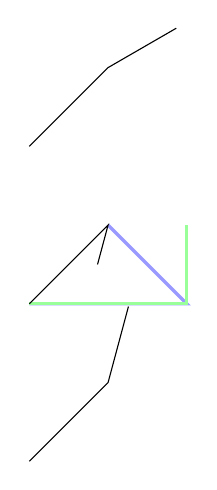
\begin{tikzpicture}
    % +(0,1)为相对于当前坐标点的坐标,但不更新到当前坐标点. 以下坐标为(0,0) (1,0) (2,0) (1,1)
    \draw[blue!40,very thick] (0,0) -- (1,0) -- +(1,0) -- +(0,1); 

    % ++(0,-1)为相对于当前坐标点的坐标,并且更新到当前坐标点. 以下坐标为(0,0) (1,0) (2,0) (2,1)
    \draw[green!40,very thick] (0,0) -- (1,0) -- ++(1,0) -- ++(0,1); 
    
    % ++(30:2)将极坐标与相对坐标结合
    \draw (0,2) -- (1,3) -- ++(30:1);
    
    % ([turn]30:1)极坐标相对于上一个点作为起始点,并且以上一个点的切线作为起始角度
    \draw (0,0) -- (1,1) -- (30:1);
    \draw (0,-2) -- (1,-1) -- ([turn]30:1);
\end{tikzpicture}\vspace{1cm}


% 命名坐标点
\begin{tikzpicture}
    \coordinate (A) at (-1,-1);
    \coordinate (B) at (-1,1);
    \coordinate (C) at (1,1);
    \coordinate (D) at (1,-1);
    \draw[->] (-2,0) -- (2,0) node[right] {$x$};
    \draw[->] (0,-2) -- (0,2) node[above] {$y$};
    \draw (A) -- (B) -- (C) -- (D) -- cycle;
\end{tikzpicture}\vspace{1cm}


% 利用伪随机数生成坐标点
% rand生成[-1,1]区间的随机数
\begin{tikzpicture}
    \draw[->] (-2.5,0) -- (2.5,0) node[below]{$x$};
    \draw[->] (0,-2.5) -- (0,2.5) node[left]{$y$};
    \foreach \x in {-2,-1,1,2}
      \draw (\x,0) node[below]{$\x$} -- (\x,2pt);
    \foreach \y in {-2,-1,1,2}
      \draw (0,\y) node[left]{$\y$} -- (2pt,\y);
    \coordinate (A) at (2*rand,2*rand);
    \fill (A) circle [radius=2pt];
\end{tikzpicture}\vspace{1cm}


% (p |- q)
% 分别取坐标p的x值,坐标q的y值,组成(x,y)
% (p -| q)
% 分别取坐标p的y值,坐标q的x值,组成(x,y)
begin{tikzpicture}[line width=0.6pt]
    \draw[help lines] (-2,-2) grid (2,2);
    \draw[->] (-2.5,0) -- (2.5,0) node[below]{$x$};
    \draw[->] (0,-2.5) -- (0,2.5) node[left]{$y$};
    \fill[red] (0,0 -| 1,1) circle [radius=2pt];
\end{tikzpicture}\vspace{1cm}


\begin{tikzpicture}
    % 线条与线条的交点,需要使用intersections库
    \path [draw,name path=x axis](-2,0) -- (2,0);
    \path [draw,name path=y axis](0,-2) -- (0,2);

    % of参数,相交的两条路径, 格式为<path_01> and <path_02>
    % by参数,相交点的坐标,可使用{}限定多个相交点
    % name参数,相交点的名称,用于后续变量引用
    % total参数,总的交点数量
    % sort by参数,指定排序依据路径
    % 交点引用格式: <name>-<num>
    \path [name intersections={of=x axis and y axis,by=G}];
    \fill (G) circle(2pt);
\end{tikzpicture}\vspace{1cm}


\begin{tikzpicture}
    % 复杂计算. section 94
    \draw (0,0) circle [radius=2];
    % \pgfmathparse{<complex_calculate>}
    %   进行复杂计算(包含函数等),将所有带单位的数字转化为pt,结果截去单位,为无单位数字
    %   将结果保存到\pgfmathresult
    %   其他简单计算会保留pt单位
    % \pgfmathresult
    %   将上一次\pgfmathparse计算结果进行引用
    \pgfmathparse{sqrt(3)}
    \coordinate (A) at (1,\pgfmathresult);
    \filldraw (A) circle [radius=2pt];

    % \pdfmathsetmacro{\<var_name>}{<complex_calculate>}
    %   复杂计算,并将计算结果保存到指定变量,结果为无单位数字
    \pgfmathsetmacro{\mdimen}{sqrt(3)}
    \coordinate (B) at (-1,\mdimen);
    \filldraw (B) circle [radius=2pt];

    % {<complex_calculate>}也可适用于复杂计算
    \coordinate (C) at (1,{-sqrt(3)});
    \filldraw[fill=green] (C) circle [radius=2pt];

    % 常用运算
    % <num>!
    %     指定数字的阶乘
    % <num> r
    %     将弧度转化为角度
    % 常用函数
    % sqrt(<num>)
    %     求平方根
    % sin(<degree>)
    %     求正弦值
    %     三角函数系列的参数必须为角度格式
    % asin(<val>)
    %     求反正弦值, 值域[-90,90]
    %     返回值为角度值  
    % atan(<val>)
    %     求反正切值
    % atan2(y,x)
    %     求y/x的反正切值
    % round(<val>)
    %     四舍五入取整数
    % floor(<val>)
    %     向下取整数
    % ceil(<val>)
    %     向上取整数
    % veclen(<len_x>,<len_y>)
    %     向量长度
\end{tikzpicture}\vspace{1cm}


\begin{tikzpicture}[>=stealth,line width=0.6pt]
    % ($<factor>*<coordinate><modifiers>$)
    % 如果提供factor,则将factor传递给\pgfmathparse进行负责计算, 需要调用calc库(section 13.5). 优化版本: 
    % {<factor>}*<coordinate><modifiers>,可更清晰区分factor和coordinate边界

    % 格式1: <factor_01>*(<coordinate_01>)+<factor_02>*(<coordinate_02>)
    % 进行坐标运算

    % 格式2: <point_start>!<percent>!<point_end>
    % 沿着point_start到point_end线段,指定百分比位置,percent可以小于0,也可以大于1
    % percent传递给\pgfmathparse计算

    % 格式3: <point_start>!<percent>!<angle>:<point_end>
    % 绕起始点point_start旋转指定角度angle,然后从结果线段上截取指定百分比位置

    % 格式4: <point_start>!<dimension>!<point_end>
    % 沿着point_start到point_end直线,距离起始点point_start长度为dimension的位置

    % 格式5: <point_start>!<dimension>!<angle>:<point_end>
    % 绕起始点point_start旋转指定角度angle,然后从结果线段上截取距离起始点长度为dimension的位置

    % 格式6: <point_start>!<point>!<point_end>
    % 由点<point>,到由<point_start>和<point_end>组成的线段的垂足

    % 格式7: <point_start>!<point>!<angle>:<point_end>
    % 由<point_start>和<point_end>组成的线段,旋转指定角度angle后,过点point到该线段的垂足
    \draw[->] (-3,0) -- (3,0) node[below]{$x$};
    \draw[->] (0,-3) -- (0,3) node[left]{$y$};
    \draw[help lines] (-2,-2) grid (2,2);
    \coordinate (A) at (1,1);
    \coordinate (B) at (2,3);
    \coordinate (C) at ($(A)+0.5*(B)$);
    \fill[red!40] (A) circle [radius=1.2pt];
    \fill[blue!40] (B) circle [radius=1.2pt];
    \fill[green!40] (C) circle [radius=1.2pt];
    \coordinate (D) at ($(A)!0.5!(B)$);
    \draw (A) -- (B);
    \fill[purple!40] (D) circle [radius=1.2pt];
\end{tikzpicture}\vspace{1cm}


% 切线系统
% (tangent cs:node=<name>,point={(<point>)},solution=<num>)
%   过一点作指定node的切线
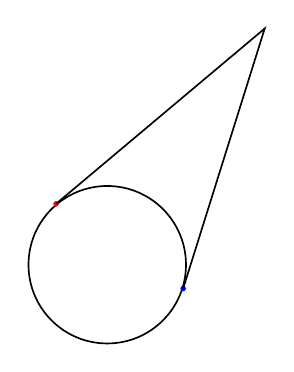
\begin{tikzpicture}[line width=0.6pt]
    \node[draw,circle,minimum size=2cm] (A) at (0,0){};
    \coordinate (P) at (2,3);
    \coordinate (M) at (tangent cs:node=A,point={(P)},solution=1);
    \coordinate (N) at (tangent cs:node=A,point={(P)},solution=2);
    \fill[red] (M) circle [radius=1pt];
    \fill[blue] (N) circle [radius=1pt];
    \draw (M) -- (P) -- (N);
\end{tikzpicture}\vspace{1cm}

% update 2025-04-17




\begin{tikzpicture}
    % 直接对坐标点进行移动_1
    \coordinate (A) at (0,0);
    \coordinate (B) at (3,0);
    \coordinate (C) at ([shift=(B)]A);
    \coordinate (D) at ([shift={(3,0)}]A);
    \draw (A) -- (C);
\end{tikzpicture}\\\vspace{1cm}

\begin{tikzpicture}
    % 直接对坐标点进行移动_2
    \draw[-stealth] (-2,0) -- (2,0) node[pos=1,below]{$x$};
    \draw[-stealth] (0,-2) -- (0,2) node[pos=1,right]{$y$};
    \foreach \x in {-1.5,-1,-0.5,0.5,1,1.5}
        \draw (\x,0) -- (\x,2pt);
    \foreach \y in {-1.5,-1,-0.5,0.5,1,1.5}
        \draw (0,\y) -- (2pt,\y);
    \filldraw (0,0) circle [radius=1.2pt];
    \filldraw ([rotate around={-90:(0.5,0)}]1,0) circle [radius=1.2pt];
\end{tikzpicture}
\end{document}
